\chapter{Massive Star Formation}
\label{ch:massivestar}

\marginnote{
\textbf{Suggested background reading:}
\begin{itemize}
\item \href{http://adsabs.harvard.edu/abs/2014prpl.conf....3D}{Tan, J.~C., et al. 2014, in "Protostars and Planets VI", ed.~H.~Beuther et al., pp.~149-172} \nocite{tan14a}
\end{itemize}
\textbf{Suggested literature:}
\begin{itemize}
\item \href{http://adsabs.harvard.edu/abs/2013ApJ...766...97M}{Myers, A.~T., et al. 2013, ApJ, 766, 97} \nocite{myers13a}
\end{itemize}
}

This chapter will focus on the particular problem of massive stars. While this might seem something of a digression from our march to ever-smaller scales, we are only prepared to address massive stars now because before tackling massive stars, we first needed to develop a theory for low-mass star formation. Only with that understanding in place are we prepared to tackle the significantly more difficult problem of how massive stars form. These stars are extremely rare -- those above 10 $\msun$ constitute only about $10\%$ of all stars formed by mass, and only about $0.2\%$ by number -- but their huge energetic output gives them an importance disproportionate to their numbers. As we shall see, this energetic output also creates unique questions regarding the process by which massive stars form.

\section{Observational Phenomenology}

\subsection{Challenges}

Unfortunately, our observational knowledge of massive star formation is much more limited than our knowledge of the analogous processes governing the formation of Solar mass stars stars. The difficulty is four-fold. First, because massive stars are rare, purely on statistical grounds locations of massive star formation are likely to be much further from Earth than sites of low mass star formation. Indeed, the nearest region of massive star formation, in the Orion cloud, is 400 pc away. Many regions of study are even further, typically $1-2$ kpc. The largest clusters, where massive star formation is most active, are located in the great molecular ring at 3 kpc from the Galactic center, about 5 kpc from us. In contrast, many of the best studied regions of low mass star formation, such as the Taurus cloud, are only $\sim 100-150$ pc from Earth. The larger distance means that we can resolve only large physical scales, and that we need proportionally more telescope time to do so.

This unfortunately compounds the second challenge: crowding and confusion. Massive stars are generally found in massive star clusters. Whether this is a physical necessity or simply a result of statistics -- i.e., can massive stars only form in clusters, or is it simply improbable that a small cluster will harbor a very rare, massive star -- is a matter of hot debate. Regardless of the outcome of that debate, the clustered environment means that extreme spatial resolution is needed to avoid confusion. For example, at the center of the Orion Nebula Cluster, where the Trapezium stars are located, the stellar density is $\sim 10^5$ pc$^{-3}$ \citep{hillenbrand98a}, so the typical interstellar distance is only $0.02$ pc, or about 5000 AU. In terms of angular resolution, at the 400 pc distance to Orion this is about $10"$. The same cluster at the distance of 2 kpc has a mean angular separation between stars at its center of $2"$. Such resolutions are in reach for the highest resolution radio and sub-mm interferometers, and in the optical from HST or ground-based systems with adaptive optics, but are not far from the limits. This means that confusion is a constant worry.

The third challenge is obscuration. As we shall see, the typical region of massive star formation has a surface density of $\sim 1$ g cm$^{-2}$. For a standard Milky Way extinction curve, including the effects of ice mantles on the dust grains, this corresponds to visual extinction $A_V\approx 500$ mag. Even in the near-infrared at K band, the extinction is only a factor of $\sim 10$ smaller, so $A_K\approx 50$ mag. This means that optical and even near-IR observations are fairly useless until the tail end of the star formation process, when the vast majority of the gas has been cleared away. Only mid-IR or radio and sub-mm observations are possible during most of the star formation process. This limitation to long wavelengths of course compounds the problem of confusion, since it means that we can get high resolution only via radio interferometers.

The final problem is timescales. As discussed in Chapter \ref{ch:feedback}, feedback from massive stars rapidly destroys the environment in which they form. For example, once they become optically revealed, the disks around massive stars probably survive $\lesssim 10^5$ yr, as opposed to $>10^6$ yr for low mass stars (as we will discuss in chapter \ref{ch:late_disk}). Thus we have a very limited window in which we can observe massive star formation underway. We essentially can only see massive star formation happening when it is still in the embedded phase. In terms of our classification scheme, massive stars only have a class 0 and a class I phase, not the longer class II or class III phases.

\subsection{Massive Clumps}

Given these challenges, what do we know? Observational surveys usually find sites of massive star formation by exploiting one of three techniques. First, such sites have huge far-IR fluxes, due to the copious amounts of warm dust that are produced by an obscured massive star. Second, sites of massive star formation are characterized by having very high surface densities, such that they are opaque at near-IR wavelengths. One can also detect these regions in near-IR absorption against the galactic background, for example using the 8 $\mu$m band on \textit{Spitzer}. The classes of object discovered this way are called infrared dark clouds (IRDCs). Figure \ref{fig:irdc_rathborne05} shows an example. Third, one can look for the maser emission that often accompanies massive star formation. The maser emission comes from strong shocks in high density gas, which are probably produced by the outflows of massive stars travelling at speeds up to $\sim 1000$ km s$^{-1}$ -- the escape speed from the stellar surface. Maser emission is useful for surveys, because masers have an immense brightness temperature, making it possible to survey the sky rapidly.

The typical clump forming a massive star cluster, detected with any technique, seems to have a mass of a few thousand $\msun$, and a radius of $\sim 1-2$ pc. Combining these numbers, the surface density is $\sim 0.1-1$ g cm$^{-2}$. This much higher that the typical surface density in regions of low mass star formation, which is generally closer to $\sim 0.01 - 0.1$ g cm$^{-2}$.  Recall from our discussion of Larson's Laws in chapter \ref{ch:gmcs} that the statement that clouds have uniform surface density is equivalent to the combination of virial balance and the linewidth-size relation. The higher surface density of massive star-forming regions compared to the bulk of the material in GMCs implies either that these regions are not in virial balance, that they are not on the linewidth-size relation, or both. When we observe these regions using a molecular tracer, for the most part we find that these clumps {\it do} appear to be roughly virial, but that they are off the linewidth-size relation seen for other material in molecular clouds.

The origin of these large velocity dispersions is an interesting problem. They could be driven by gravitational collapse, of course, but that would only supply energy for one crossing time or so, and then would lead to global collapse. We know from galactic-scale surveys, however, that this gas cannot form stars rapidly any more than can the lower density material in GMCs. Otherwise the star formation rate would be too high to compared to what we observe. This suggests that these regions must be stabilized by internal feedback or disrupted by feedback in only $\sim 1$ crossing time, before they have the opportunity to convert most of the gas mass to stars.

\begin{figure}
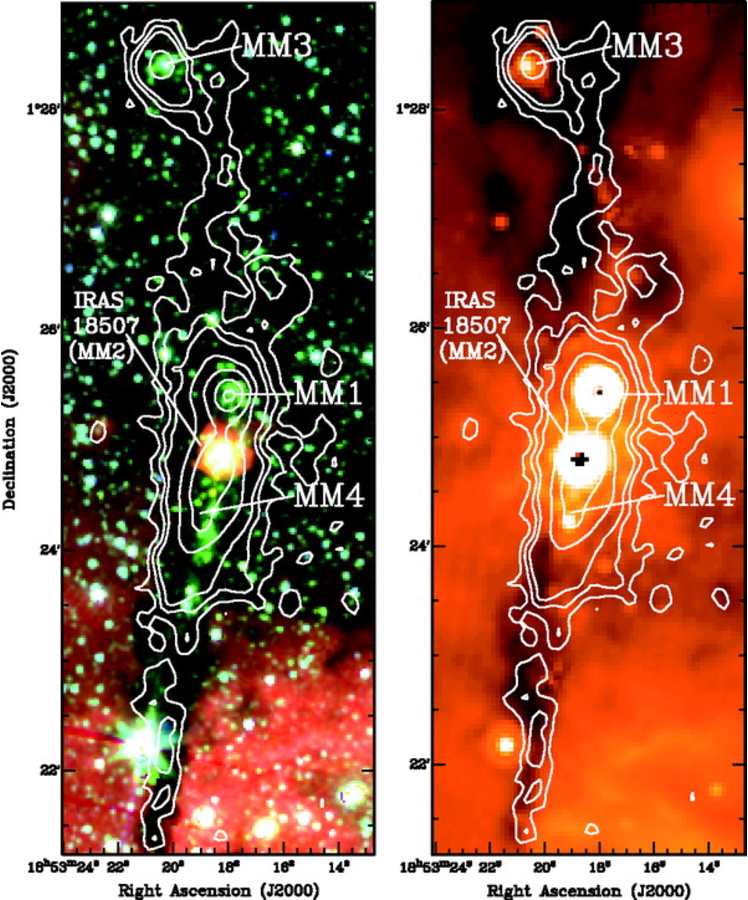
\includegraphics[width=\linewidth]{irdc_rathborne05}
\caption[IR and mm images of an IRDC]{
\label{fig:irdc_rathborne05}
A typical infrared dark cloud (IRDC) \citep{rathborne06a}. The left image shows \textit{Spitzer}/IRAC (near-IR), where the cloud is seen in absorption against the galactic background, while the right image shows \textit{Spitzer}/MIPS (mid-IR), where parts are seen in absorption and parts in emission. The white contours, which are the same in both panels, show mm continuum emission from cold dust.
}
\end{figure}


\subsection{Massive Cores}
\label{ssec:massivecores}

If one zooms in a bit more using an interferometer, to $\sim 0.1$ pc scales, one can find objects that are $\sim 100$ $\msun$ in mass and $\sim 0.1$ pc in radius. These are centrally concentrated, and appear to be forming stars. Their velocity dispersions are also about one is needed for them to be in virial balance, around 1 km s$^{-1}$. As with their parent clumps, such large velocity dispersions on such small scales puts these objects well off the linewidth-size relation seen in most material in GMCs. We refer to objects with these characteristics as massive cores. Figure \ref{fig:massivecore_butler12} shows an example.
\begin{marginfigure}
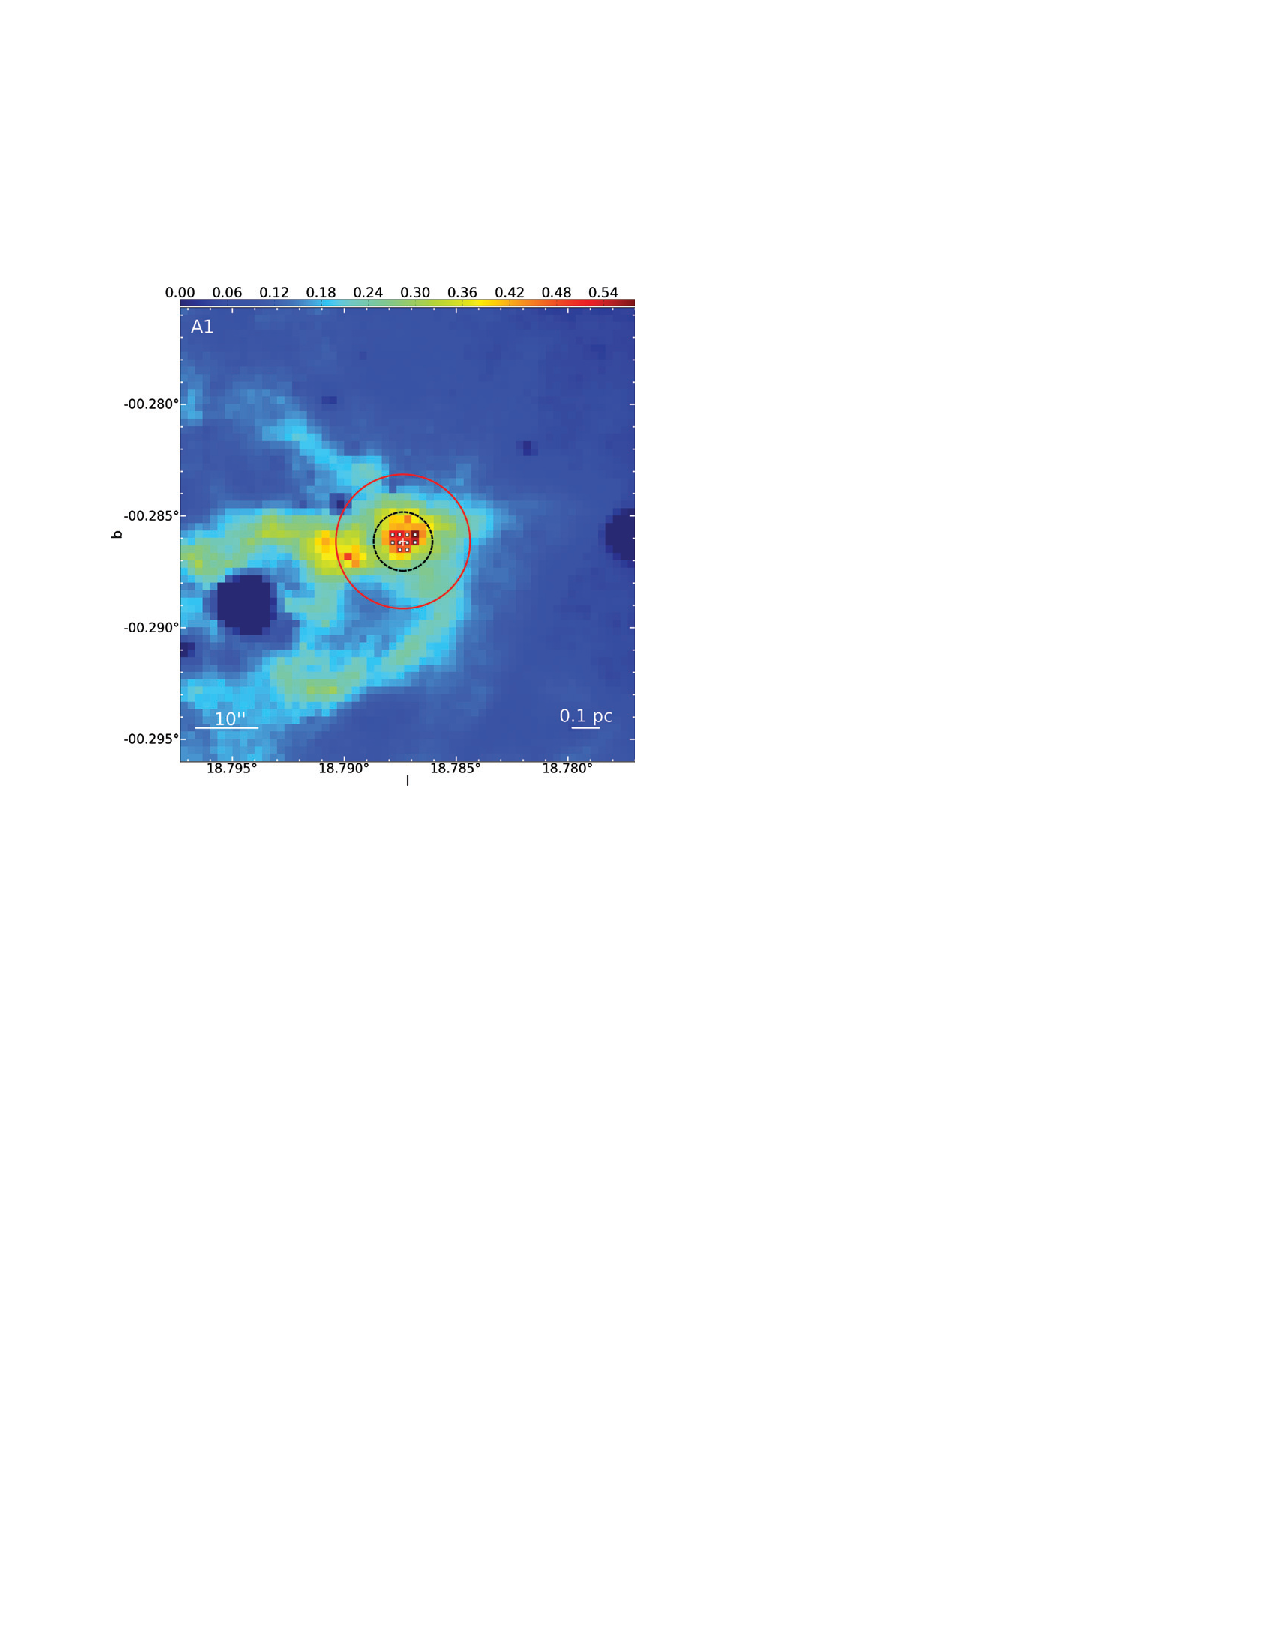
\includegraphics[width=\linewidth]{massivecore_butler12}
\caption[A massive core in IR absorption]{
\label{fig:massivecore_butler12}
A massive protostellar core seen in IR absorption \citep{butler12a}. Colors indicate the inferred column density in g cm$^{-2}$. Pixels marked with white dots are lower limits. The black circle shows a radius enclosing $60$ $M_\odot$, and the red circle shows the core radius inferred by fitting a core plus envelope model to the azimuthally-averaged surface density distribution.
}
\end{marginfigure}

In some cases we detect no mid-IR emission from massive cores, which indicates that any stars within them cannot yet be massive stars. However, even in cases with no mid-IR, there are signs of active protostellar outflows, in the form of SiO emission \citep[e.g.,][]{motte07a}. The statistics indicate that the starless phase for a massive core is at most $\sim 1000$ yr, implying that once a massive core is assembled it starts forming stars immediately, or even that star formation begins as it is being assembled.

It is instructive to perform some simple dimensional analysis for these objects. A region with a mass of $100$ $\msun$ and a radius of $0.1$ pc has a mean density of about $10^{-18}$ g cm$^{-3}$, or $n\sim 10^6$ cm$^{-3}$, and a free-fall time of $5\times 10^4$ yr. Thus we should expect one of these cores to form stars in $\sim 10^5$ yr, and to do so at an accretion rate $\dot{M}\approx M/t_{\rm ff} \approx 10^{-3}$ $\msun$ yr$^{-1}$. This is vastly higher than the expected accretion rates in the regions of low mass star formation close to Earth, and much larger than $c_s^3/G$ where $c_s$ is the thermal sound speed. 

It is also useful to phrase the accretion rate in terms of a velocity dispersion. Suppose we have a core in rough virial balance, so that
\begin{equation}
\alpha_{\rm vir} = \frac{5 \sigma^2 R}{G M} \approx 1,
\end{equation}
where the 1D velocity dispersion $\sigma$ here now includes contributions from both thermal and non-thermal motions. The density is $\rho=3 M/(4\pi R^3)$, so the free-fall time is
\begin{equation}
t_{\rm ff} = \sqrt{\frac{3\pi}{32 G \rho}} = \sqrt{\frac{\pi R^3}{8 G M}}.
\end{equation}
If the core collapses in free-fall, the accretion rate is
\begin{equation}
\dot{M} \approx \frac{M}{t_{\rm ff}} = \sqrt{\frac{8 G M^3}{\pi R^3}} = \sqrt{\frac{1000}{\pi\alpha_{\rm vir}^3}} \frac{\sigma^3}{G}.
\end{equation}
Thus, the accretion rate will be roughly $\sim 10 \sigma^3/G$.

\section{Fragmentation}

\subsection{Massive Core Fragmentation}

Given that we see these massive cores, can we understand how they turn into massive stars? The first thing that happens when one of these cores begins to collapse is that it will be subject to fragmentation. In effect, because it is so much larger than a thermal Jeans mass, a 100 $\msun$ massive core has the potential to become a small cluster rather than a single star or star system. On the other hand, both radiative heating and magnetic fields are capable of suppressing fragmentation. So what happens?

This still a very active area of research, but recent simulations by \citet{commercon11c} and \citet{myers13a} that explore how radiative transfer and magnetic fields affect star formation suggests that a combination of the two is very effective at suppressing fragmentation of massive protostellar cores. The basic mechanism is quite analogous to the way that radiation feedback can shape the IMF overall: rapid accretion gives rise to a high accretion luminosity, which in turn heats the gas and raises the Jeans mass. Magnetic fields enhance this effect in two ways. First, by providing a convenient way of getting rid of angular momentum (as discussed in chapter \ref{ch:disks_theory}), they enhance the accretion rate. Second, they tend to stabilize the more distant, cooler parts of the core that are less heated by the radiation. These low-density regions may be Jeans unstable, but they are also magnetically subcritical and thus cannot fragment and collapse. Figure \ref{fig:msf_myers13} shows an example simulation.

\begin{figure}
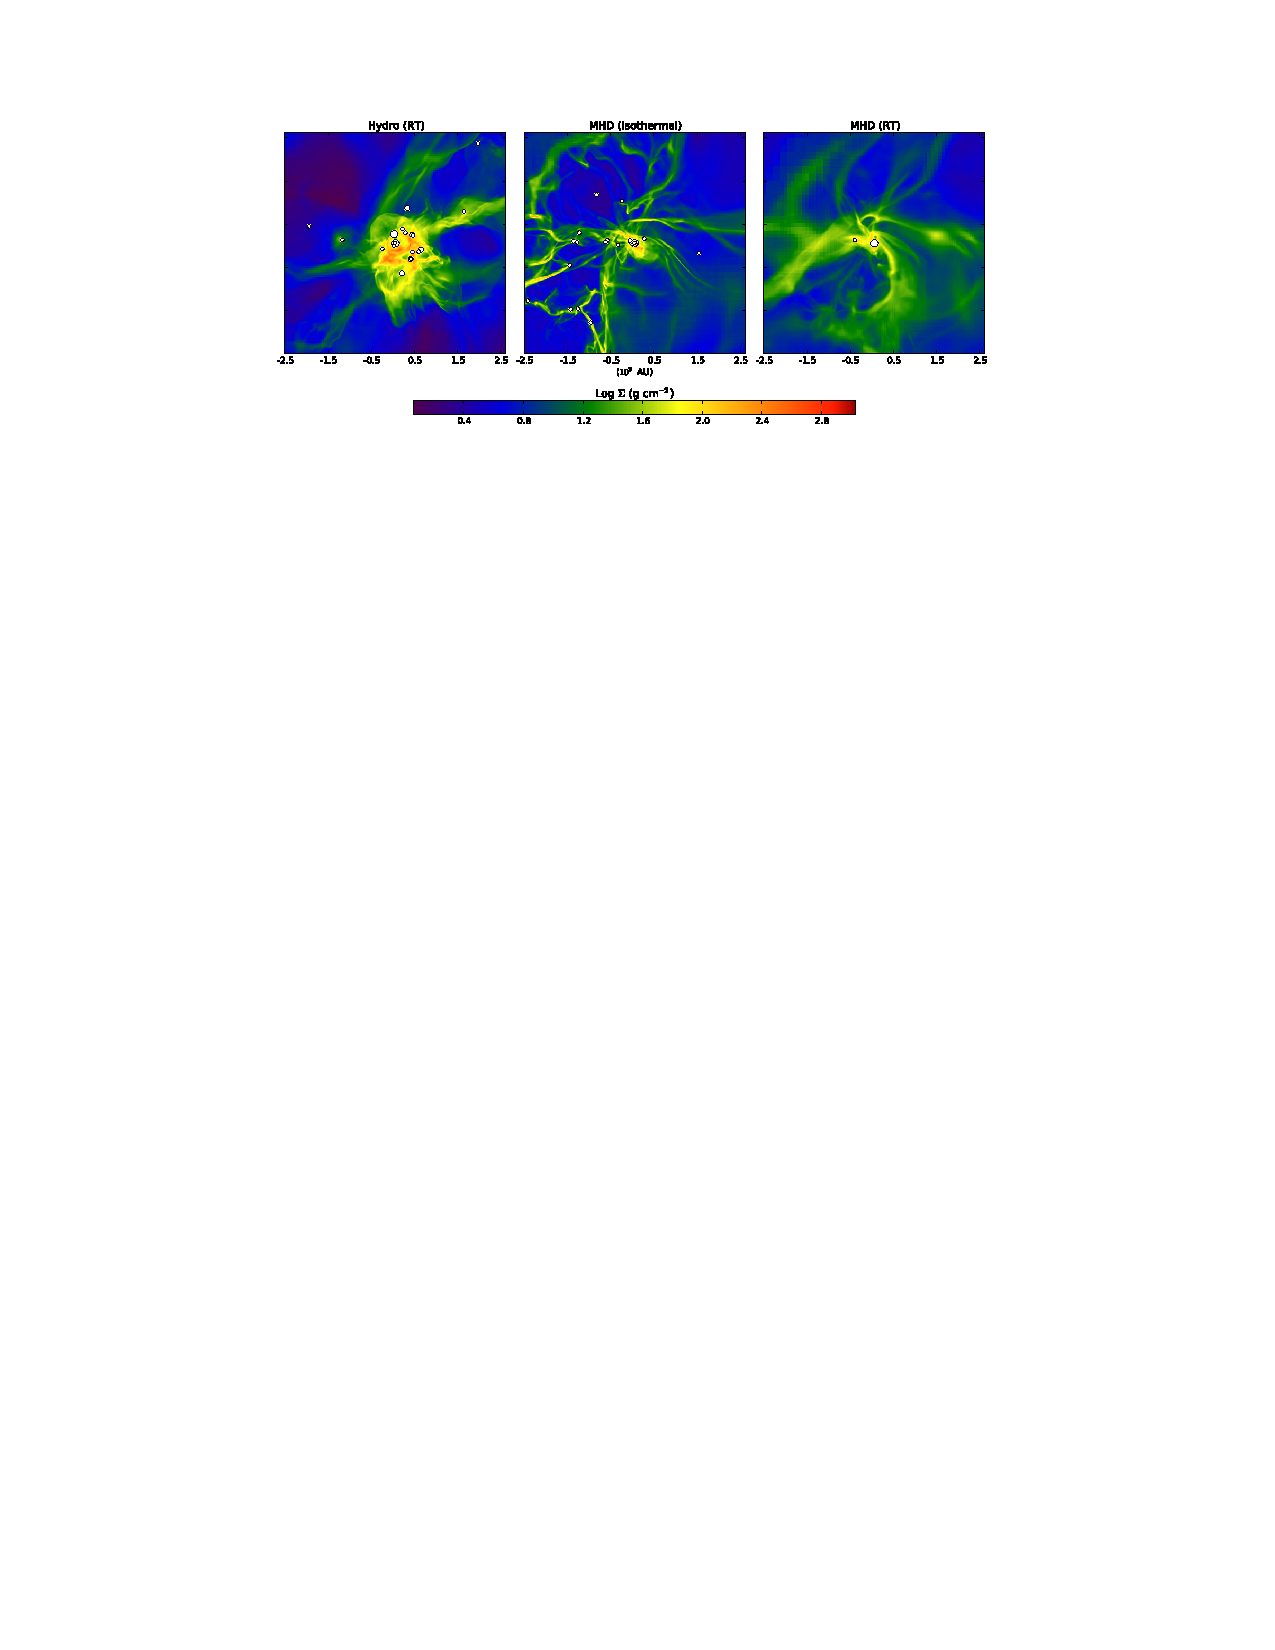
\includegraphics[width=\linewidth]{msf_myers13}
\caption[Simulations of massive star formation with magnetic fields and radiation]{
\label{fig:msf_myers13}
Three simulations of the collapse of a 300 $M_\odot$ massive core by \citet{myers13a}. The color scale shows the projected gas density, and white points are stars, with the size indicating the mass. The three simulations use identical initial conditions, but different physics. The left panel uses radiative transfer but no magnetic fields, the middle uses magnetic fields but no radiation, and the right panel includes both magnetic fields and radiation.
}
\end{figure}

\subsection{Massive Binaries}

As discussed in chapter \ref{ch:imf_obs}, massive stars are overwhelmingly members of binary or higher multiple star systems. Why this should be is obviously an interesting question, and related to the topic of fragmentation. Binaries can form in two ways. One way of making binaries is what we can call direct fragmentation: a collapsing gas core breaks up into two or more pieces during collapse. This possibility is closely related to the discussion of the IMF, in that it depends on the thermodynamics of the gas and its turbulent motions. The other possibility is disk fragmentation, in which material collapses into a disk and that disk then fragments. Direct fragmentation almost has to be the origin for wide period binaries, those with separations $\gtrsim 1000$ AU, the typical size of a protostellar disk. It could also be the origin for close ones. However, it is suggestive that the mass ratio distribution is somewhat different for close binaries than for distant ones.

There have been several numerical studies of the circumstances under which a core is expected to undergo fragmentation to produce a binary. Generally speaking, the amount of fragmentation appears to depend on the amount of initial turbulence in the core. Two important parameters controlling when and whether this happens are rate of rotation and the strength of the magnetic field in the initial cloud. A third parameter that becomes relevant in disks is the relationship between gas density and temperature.

\citet{machida08b} varied the rotation rate and magnetic field strength in clouds and found that they could draw boundaries in parameter space determining where various types of fragmentation occur. Higher rotation rates and weaker magnetic fields favor direct fragmentation, while slower rotation rates and stronger magnetic fields favor no fragmentation. Disk fragmentation appears to occur at intermediate values. Of course real cores have some level of turbulence, even if they are subsonic, and it is not entirely clear how to translate these conditions into probabilities of binary formation for turbulent cores.

The nature of disk fragmentation and its relationship with the thermal properties of the gas has been clarified in a series of papers by \citet{kratter06a} and \citet{kratter08a, kratter10a}. These authors point out that the behavior of a collapsing, rotating, non-magnetic core can be described in terms of two dimensionless numbers:
\begin{equation}
\xi \equiv \frac{\dot{M} G}{c_s^3} \qquad\qquad \Gamma = \frac{\dot{M}}{M_{*d}\Omega_{k,\rm in}} = \frac{\dot{M} \langle j\rangle_{\rm in}}{G^2 M_{*d}^3}.
\end{equation}
Here $\dot{M}$ is the rate at which matter falls onto the edge of the disk, $c_s$ is the sound speed in the disk, $M_{*d}$ is the total mass of the disk and the star it orbits, $\Omega_{k,\rm in}$ is the Keplerian angular frequency of matter entering the disk and $\langle j\rangle_{\rm in}$ is the mean specific angular momentum of matter entering the disk.

The meanings of these two dimensionless numbers are straightforward. The first, $\xi$, takes the ratio of the accretion rate to the characteristic thermal accretion rate $c_s^3/G$. This is (up to factors of order unity) the accretion rate for a singular isothermal sphere or a Bonnor-Ebert sphere, and it is also the characteristic accretion rate through an isothermal disk, as we will see in Chapter \ref{ch:disks_theory}. The second parameter, $\Gamma$, is a measure of the angular momentum content of the accretion. The quantity $\dot{M}/\Omega_{k,\rm in}$ is (neglecting a factor of $2\pi$) the amount of mass added per orbital period at the disk outer edge. Thus $\Gamma$ measures the fraction by which accretion changes the total disk plus star mass per disk orbital period. High angular momentum flows have large rotation periods, so they produce larger values of $\Gamma$ at the same total accretion rate.
\begin{marginfigure}
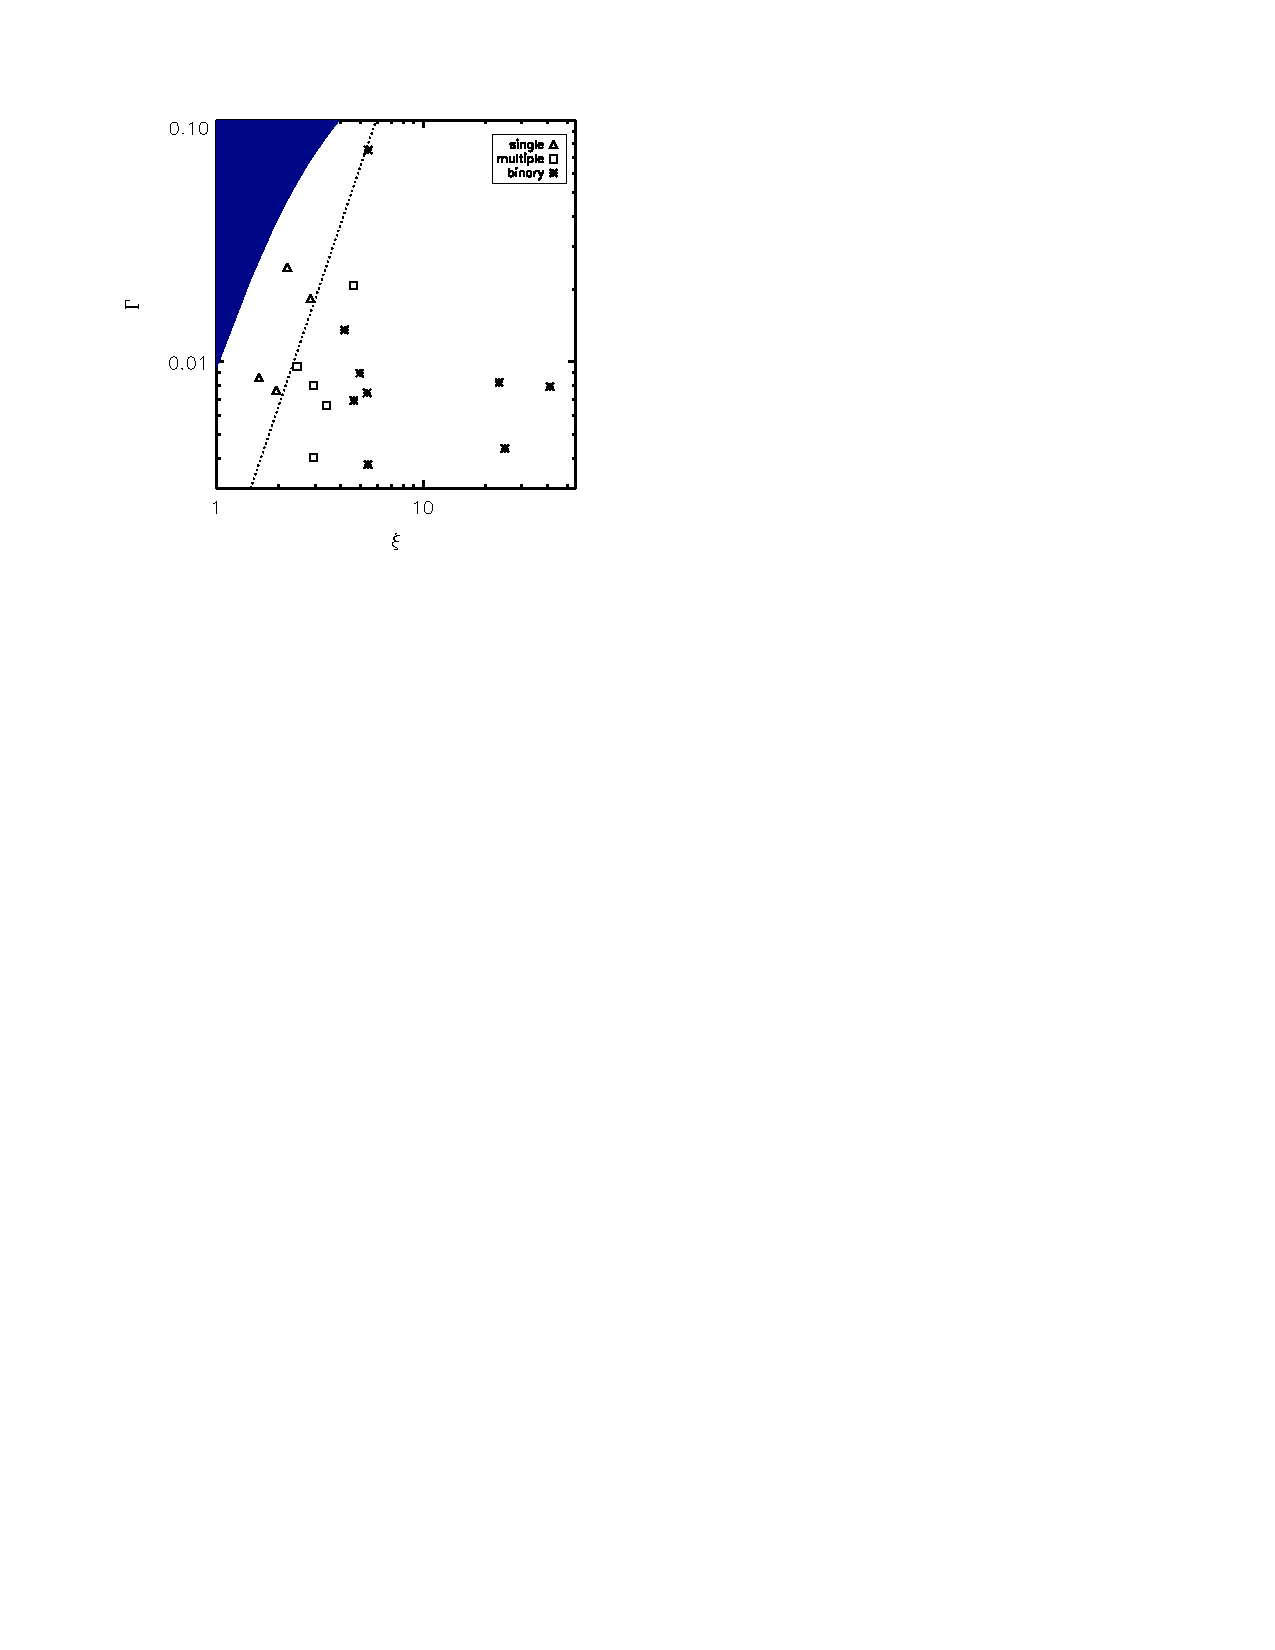
\includegraphics[width=\linewidth]{diskfrag_kratter10}
\caption[Parameter study of disk fragmentation]{
\label{fig:diskfrag_kratter10}
Results of a series of simulations of disk fragmentation by \citet{kratter10a}. Points show the accretion rate parameter $\xi$ and the rotation parameter $\Gamma$ for the simulations, with the type of point indicating the outcome: a single star, a multiple system, or a binary system. The shaded region is forbidden, because cores in that region are unable to collapse.
}
\end{marginfigure}

Intuitively, we expect that disk fragmentation is likely for high values of $\xi$ and low values of $\Gamma$, because both favor higher surface densities in the disk. High $\xi$ favors high disk surface density because it corresponds to matter entering the disk faster, and low $\Gamma$ favors higher surface density because it tends to make the disk more compact (since the circularization radius of the accreting material increases and $\Gamma$ does). This is exactly what a series of numerical simulations shows, as illustrated in Figure \ref{fig:diskfrag_kratter10}.

These results are very nice because they quite naturally explain why binaries are much more common among high mass stars. We showed in Section \ref{ssec:massivecores} that typical accretion rates onto massive stars are $\sim 10 \sigma^3/G$, where $\sigma$ is the velocity dispersion in the protostellar core. The parameter $\xi$ is determined by the accretion rate normalized to $c_s^3/G$ (where $c_s$ is the disk sound speed, recall), and thus we have
\begin{equation}
\xi \sim 10\left(\frac{\sigma}{c_s}\right)^3.
\end{equation}
For a massive core, the disk sound speed $c_s$ is enhanced compared to that in the core due to the radiation from the star, but much less than $\sigma$ is enhanced. Typical outer disk temperatures for massive star disks are $\sim 100$ K, corresponding to $c_s \sim 0.6$ km s$^{-1}$, whereas $\sigma \sim 1$ km s$^{-1}$, giving $\xi \gg 1$. Thus disk fragmentation is essentially inevitable.

A second effect that enhances massive star binary is N-body processing. Young clusters are born far from dynamically-relaxed, and thus there is an initial period where stars may have close encounters with one another. During this phase, encounters between binary systems, between binaries and single stars, and between three single stars can all serve to create or destroy binaries, or to modify their properties. The study of exactly how this happens is a huge topic into which we will not delve, beyond making a few general observations.

The main effects of this N-body processing are as follows: (1) wide binaries will tend to be widened and disrupted; (2) tight binaries will tend to get tighter; (3) three-body interactions may occur that will tend to preferentially keep more massive stars in binaries, thus favoring equal mass ratios. The line between close and wide binaries depends on the velocity -- binaries with orbital velocities greater than the cluster velocity dispersion are close, others are wide. All of these effects will tend to increase the binary fraction for more massive stars relative to less massive ones; the third effect does so by creating new massive binaries, and the first two favor massive binaries because a higher mass produces a higher orbital velocity, and thus a wider range of separations that can be considered close.

\section{Barriers to Accretion}

\subsection{Evolution of Massive Protostars}

Massive stars are not only somewhat different from low mass stars in terms of their parent cores, but also in their internal evolution. At accretion rates of $\sim 10^{-4}-10^{-3}$ $\msun$ yr$^{-1}$, forming a $10-100$ $\msun$ star takes of order $10^5$ yr, not that different than the time require to make a low mass star. However, massive stars are very different than low mass ones in terms of the timescales that govern their thermal evolution. As discussed in chapter \ref{ch:protostar_evol}, the characteristic timescale on which a star will contract toward the main sequence is the Kelvin-Helmholtz timescale
\begin{equation}
t_{\rm KH} = \frac{GM^2}{RL}.
\end{equation}
Evaluating this for main sequence values of $M$, $R$, and $L$, for a zero age main sequence (ZAMS) star of mass $1$ $\msun$, $t_{\rm KH} = 50$ Myr.  For a protostar where $R$ and $L$ are both larger (see chapter \ref{ch:protostar_evol}), this drops to $\sim 1$ Myr. On the other hand, to put some numbers on this for a massive star, a 50 $\msun$ ZAMS star has a radius of $10.7$ $\rsun$ and a luminosity of $3.5\times 10^5$ $\lsun$. For this star $t_{\rm KH}=20$ kyr, even without putting in a larger radius because it is pre-main sequence. Since this is less than the $\sim 100$ kyr required to form the star, we expect that massive stars will be able to reach thermal equilibrium, and thus contract to the main sequence, while forming, whereas low mass stars will not.

The rapid contraction to the main sequence has a few consequences. It means that the stars will have stronger winds, since the wind speed is linked to the Keplerian speed at the stellar surface and massive stars are able to shrink more. Similarly, the stars' comparatively small radii imply is that the effective temperature will be fairly high, so much of the light will emerge as ionizing radiation, even while the star is still forming. Finally, rapid settling means that massive protostars will put out roughly the same amount of light as main sequence stars of the same mass, since they will rapidly contract down to similar sizes. This in turn means that, unlike low mass protostars, massive protostars' luminosities come primarily from internal processes and not from accretion. The accretion luminosity of a massive star is larger than that of a low mass star because both its mass and its accretion rate are larger, but this effect is swamped by the extremely strong mass-dependence of the internal luminosity, which in the vicinity of $1$ $M_\odot$ rises as roughly $L \sim M^4$. Because of this strong mass-dependence, massive stars' accretion luminosities generally become subdominant once they reach $\sim 5-10$ $M_\odot$, depending on the accretion rate. The fact that massive protostars settle onto the main sequence while forming raises interesting problems for how they are able to keep accreting.

\subsection{Winds}

One thing that one might worry about is that the main sequence winds of a massive star, which are reasonably isotropic, might inhibit accretion. These winds may well start up while the star is still forming. However, this worry is fairly easy to dismiss. Main sequence O stars show wind speeds up to $\sim 1000$ km s$^{-1}$, with mass fluxes that are typically $\sim 10^{-7}$ $\msun$ yr$^{-1}$ or less. The mass flux is
\begin{equation}
\dot{M} = 4\pi r^2 \rho v,
\end{equation}
so the associated ram pressure is
\begin{equation}
P_{\rm wind} = \rho v^2 = \frac{\dot{M}_{\rm wind} v_{\rm wind}}{4\pi r^2}.
\end{equation}
In contrast, the accretion flow has a mass flux of $10^{-4}-10^{-3}$ $\msun$ yr$^{-1}$, and if it arrives at free-fall its ram pressure is
\begin{equation}
P_{\rm infall} = \frac{\dot{M}_{\rm acc} v_{\rm ff}}{4\pi r^2}.
\end{equation}
Thus the ratio of the ram pressures is
\begin{equation}
\frac{P_{\rm infall}}{P_{\rm wind}} = \frac{\dot{M}_{\rm acc} v_{\rm ff}}{\dot{M}_{\rm wind} v_{\rm wind}}.
\end{equation}

Since $v_{\rm wind} \approx v_{\rm ff}$ at the stellar surface, and $\dot{M}_{\rm acc}$ is larger than $\dot{M}_{\rm wind}$ by a factor of $10^3-10^4$, the ram pressure of the infall is more than enough to stop the wind. Even if the wind and the infall encounter each other further from the star, the free-fall velocity only falls off as $r^{-1/2}$, so the wind would need to be able to push the infall out to $\sim 10^6-10^8$ stellar radii before it would be able to reverse the infall. For a 50 $\msun$ ZAMS star, $10^6$ stellar radii is roughly $0.25$ pc, i.e., bigger than the initial massive core.

Thus, we generally do not expect main sequence stellar winds to inhibit accretion as long as material is left in the protostellar core. Of course the protostellar outflow carries much more momentum than the main sequence wind because it is hydromagnetically rather than radiatively driven (see chapter \ref{ch:disks_theory}). However, it is also highly collimated, and so it does not prevent accretion over $4\pi$ sr any more than protostellar outflows from lower mass stars do. It will reduce the efficiency, but not by more than low mass star outflows do.

\subsection{Ionization}

A second feedback one can worry about is ionizing radiation. Massive stars put out a significant fraction of their power beyond the Lyman limit, and this can ionize hydrogen in the envelope around them. Since when hydrogen is ionized it heats up to $\sim 10$ km s$^{-1}$, gas that is ionized may be able to escape from the massive core, which only has an escape velocity of $\sim 1$ km s$^{-1}$.

This does eventually happen, and it probably plays an important role in regulating the star formation efficiency in star clusters and on larger scales. However, one can show that, as long as the massive star is accreting quickly, this effect will not limit its ability to continue gaining mass. Problem set 5 contains a quantitative calculation of this result. Foreshadowing it here, at the accretion rates that we expect in massive cores, the ionizing radiation should all be trapped within a few stellar radii of the stellar surface. Since the escape velocity from the surface of a 50 $\msun$ ZAMS star is about $1000$ km s$^{-1}$, this gas will be trapped by the star's gravity, and will not escape. Thus ionization is an important feedback, but it is one that is likely most important after the massive star has gathered most of the mass around it and has stopped growing.

That said, this omits the fact that there is likely to be lower density within the region cleared by the protostellar outflow, so ionizing radiation may be able to escape in some directions even while the star is growing. This may eventually reduce its mass supply, and it may cause asymmetric H~\textsc{ii} regions to form, where the ionized gas is confined in certain directions (for example close to the disk) while the ionizing photons escape and drive an outflow in other directions (for example along the polar axis).

\subsection{Radiation Pressure}

By far the biggest potential worry for massive star formation is not that ionizing radiation will heat the gas enough to allow it to escape, but the pressure exerted by radiation will halt accretion. Let us go back to our picture of the structure of the envelope of dusty gas around a protostar, developed in chapter \ref{ch:protostar_form}. There is a dust destruction radius where all direct starlight is absorbed, and outside that a diffusion region. The calculation of this radius is the same as for a low mass star, except that the luminosity is not mostly due to accretion. Equating heating and cooling (and again ignoring the complication introduced by dust grain sizes smaller than $\sim 1$ $\mu$m) gives
\begin{equation}
\frac{L_*}{4\pi r_d^2} \pi a^2 = 4\pi a^2 \sigma T_d^4,
\end{equation}
where $r_d$ and $T_d$ are the radius and temperature at the dust destruction front. Thus
\begin{equation}
r_d = \sqrt{\frac{L_*}{16 \pi \sigma T_d^4}} = 25\mbox{ AU}\; L_{*,5}^{1/2} T_{d,3}^{-2},
\end{equation}
where $L_{*,5} = L_*/(10^5\,\lsun)$ and $T_{d,3}=T_d/(1000\mbox{ K})$. The dust destruction radius is therefore a factor of $\sim 10$ larger than it is for a low mass star.

\paragraph{Direct radiation pressure at the dust destruction front.} It is interesting to consider the force exerted by the radiation on the gas in two different regimes. One is at the dust destruction front, where the radiation still has a stellar spectrum and has not yet been down-shifted in frequency by the dust. At this front we can assume that essentially all the stellar radiation is absorbed in a thin region, so all of the momentum carried by the stellar radiation field will be transferred to the gas. Infall will reverse if this change in momentum is enough to reduce the infall velocity to zero.

Let $\dot{M}$ be the mass accretion rate onto the star. An infalling shell of material striking the dust destruction front therefore carries an inward momentum flux
\begin{equation}
\dot{p} = -\dot{M} v,
\end{equation}
where $v$ is the material's velocity, and we use the convention that $\dot{M}>0$ and $v>0$ correspond to inward motion. In comparison, the stellar radiation field carries a momentum flux
\begin{equation}
\dot{p} = \frac{L}{c}
\end{equation}
Strictly speaking this momentum is transferred to the dust grains, since they and not the gas absorb the radiation. However, the grains are coupled to the gas by collisions and magnetic fields, so they will in turn transfer any momentum they absorb to the gas.

If we let $v_0$ be the velocity of the material just before it encounters the stellar radiation field and $v_1$ be its velocity after passing through the dust destruction front, then conservation of momentum implies that
\begin{equation}
\dot{M} v_1 = \dot{M} v_0 - \frac{L}{c}.
\end{equation}
The condition that $v_1 < 0$ (i.e., that the new velocity still be inward) then requires that
\begin{equation}
\dot{M} v_0 > \frac{L}{c}
\end{equation}
If we assume that the gas is arriving at free-fall before reaching the dust destruction front, then $v_0 = \sqrt{2 G M/r_d}$, and thus the mass flux must exceed
\begin{equation}
\label{eq:mdot_min}
\dot{M} > \frac{L}{v_0 c} = \frac{L}{c} \sqrt{\frac{r_d}{2 G M_*}} = 8\times 10^{-5} \,\msun\mbox{ yr}^{-1} \, L_{*,5}^{3/2} T_{d,3}^{-1} M_{*,1}^{-1/2},
\end{equation}
where $M_{*,1}=M_*/(10\,\msun)$.

This is less than the accretion rates we inferred for massive stars based on dimensional arguments, although maybe not by quite as much as one would like. Nonetheless, this seems to imply that matter will not be stopped at the dust destruction front if it arrives as quickly as expected. More detailed evaluations of this condition by \citet{mckee03a}, who in turn build off of \citet{wolfire87a}, generally find that this is not a problem. However, there is an important caveat to mention. In deriving equation (\ref{eq:mdot_min}), we plugged in a radius $r_d$, which assumes that the direct radiation pressure encounters the gas at $r_d$. If something is able to evacuate the gas out to a radius $r > r_d$ (for example the diffuse radiation pressure we will consider momentarily), then the infall momentum is reduced as $r^{-1/2}$, while the momentum budget of the radiation remains the same. Thus direct radiation pressure cannot halt accretion by itself, but if something else begins to evacuate the region around the star, then direct radiation pressure may be able to keep it evacuated or even expand the evacuated region.

\paragraph{Diffuse radiation pressure in the envelope.} The second regime to think about this the dusty envelope, through which radiation must diffuse to escape. The radiation flux $F=L/(4\pi r^2)$, and this applies a force per unit mass to the gas
\begin{equation}
f_{\rm rad} = \frac{1}{c} \int \kappa_{\nu} F_{\nu} \, d\nu = \frac{1}{4\pi r^2 c} \int \kappa_{\nu} F_{\nu} \, d\nu,
\end{equation}
where the subscript $\nu$ indicates the frequency-dependent flux and opacity. Since the radiation field will be close to a black body in the envelope, we can replace the frequency integral with a Rosseland mean opacity, giving
\begin{equation}
f_{\rm rad} = \frac{\kappa_{\rm R} F}{c} = \frac{\kappa_{\rm R} L_*}{4\pi r^2 c}
\end{equation}

Since the opacity of the gas to the reprocessed radiation field is much less than its opacity to direct stellar radiation (i.e., $\kappa_{\rm R}$ evaluated at temperatures $T<T_d$ is much smaller than $\kappa_{\nu}$ evaluated at the peak frequency of stellar output), this force is much less than that applied at the dust destruction front. Unlike at the dust destruction front, however, this force is not applied in a quick impulse. It is applied at every radius, and thus its cumulative effect can be much stronger than that at the dust destruction front. If we think of things in terms of accelerations, the force applied in the dust envelope is much smaller, but it is applied to the gas for a much longer time, so that the total acceleration can be larger. The relevant comparison here is not to the momentum of the radiation field, but to the force of gravity exerted by the star, since we want to know whether the net acceleration is inward or outward.

The condition that gravitational force be stronger than radiative force is
\begin{equation}
\frac{G M_*}{r^2} > \frac{\kappa_{\rm R} L_*}{4\pi r^2 c},
\end{equation}
or
\begin{equation}
\frac{L_*}{M_*} < \frac{4\pi G c}{\kappa_{\rm R}}.
\end{equation}
This is just the Eddington limit calculation, or it would be if we plugged in the electron scattering opacity for $\kappa_{\rm R}$.
If we instead plug in a typical infrared dust opacity of a few cm$^2$ g$^{-1}$, we get
\begin{equation}
\left(\frac{L_*}{M_*}\right) = 1300 (\lsun/\msun) \,\kappa_{\rm R,1}^{-1},
\end{equation}
where $\kappa_{\rm R,1} = \kappa_{\rm R}/(10\mbox{ cm}^2\mbox{ g}^{-1})$.
For comparison, our standard 50 $\msun$ ZAMS star has $L_*/M_*= 7100 (\lsun/\msun)$, and thus it exceeds this limit by a factor of $\sim 5$. In fact, all ZAMS stars larger than $\sim 20$ $\msun$ exceed the limit, which would seem at face value to suggest that it should not be possible to form stars above this limit by accretion. This argument led to all sorts of contortions trying to explain how massive stars could form -- models included trying to make them only in regions of dramatically reduced dust opacity, trying to make them by collisions of lower mass stars, and various other ideas.

The solution in reality is much more prosaic: the real world is not spherically symmetric, and the argument we just went through is. Multidimensional simulations show that, contrary to this naive calculation, radiation does not stop accretion in a real system. The main effect is that the ram pressure and the gas pressure can both be asymmetric, and they will conspire to be anti-correlated with one another because the radiation will escape by the path of least resistance. This asymmetry can be produced by many mechanisms; an obvious one is angular momentum, which shapes the accretion flow into a disk can concentrates ram pressure in a plane, while radiation pressure is not so confined. A shell of material held up by the radiation field turns out to be unstable, allowing radiation to escape asymmetrically and concentrating the infall. Magnetic fields or turbulence will both produce filamentary infall, again concentrating the ram pressure of the gas over a small solid angle, while allowing radiation to escape over the remaining, unoccupied solid angle. Outflows present yet another mechanism to punch a whole through which radiation can escape, as illustrated in Figure \ref{fig:msf_cunningham11}. For all these reasons, it is misleading to compare the radiation and gravitational forces averaged over $4\pi$ sr. Accretion will continue as long as there are significant patches of solid angle where gravity wins.

\begin{figure}
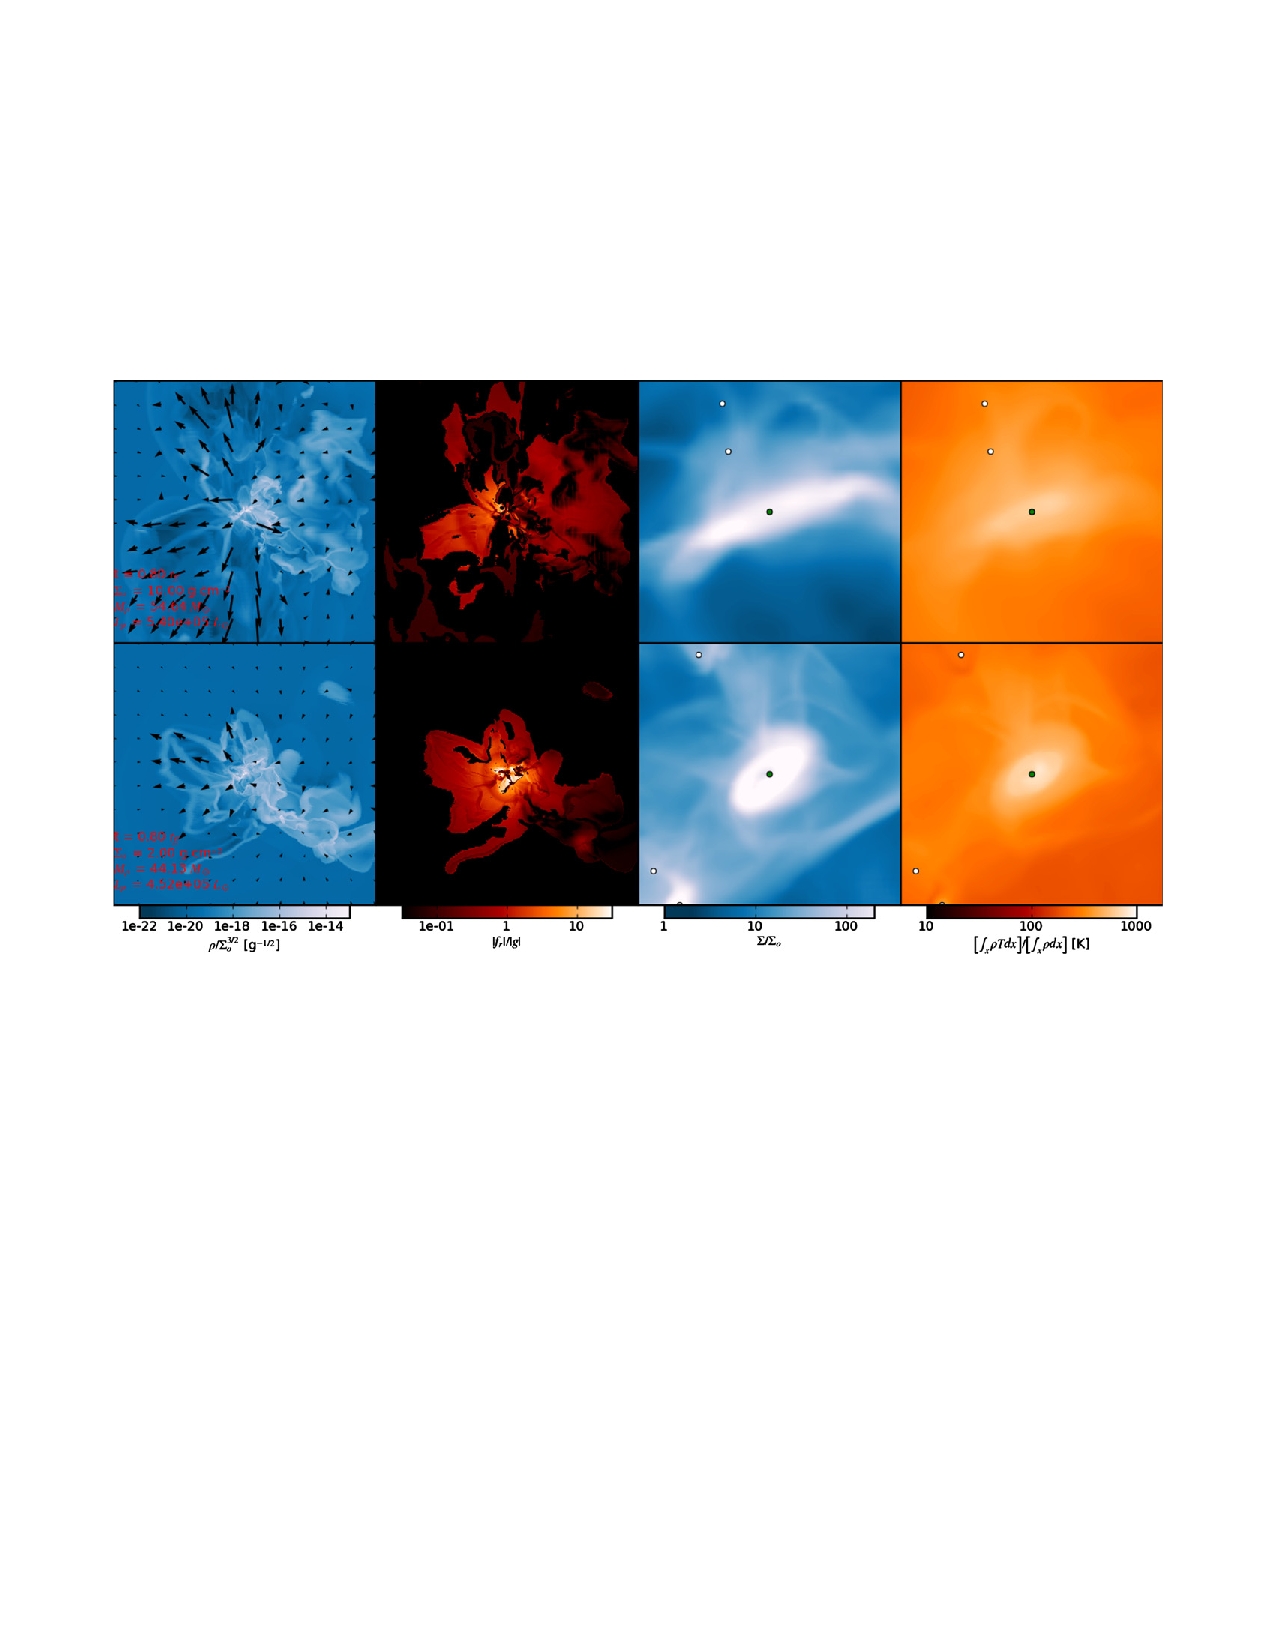
\includegraphics[width=\linewidth]{msf_cunningham11}
\caption[Simulation of massive star formation with outflows]{
\label{fig:msf_cunningham11}
Two simulations of the formation of a massive star including protostellar outflows \citep{cunningham11a}. The top row shows a simulation with an outflow, while the lower shows one without. The panels show, from left to right, normalized volume density in a slice, ratio of radiation force to gravitational force, normalized projected density, and mass-weighted mean projected temperature. Note the general absence of regions with radiation force greater than gravitational force in the simulation with winds.
}
\end{figure}

